\section{Class Diagram}

After analysing on the domain of the project, we have come up with the following class diagram.\\
It consists of four packages:
\begin{itemize}
    \item controller, which contains our controller-classes.
    \item ui, which contains a UI-interface and a TUI, which implements this.
    \item dal, which contains our data-access objects.
    \item dto, which contains our data-transfer objects.
\end{itemize}

\noindent The program starts in our \texttt{Main}-class, which has the main method. This class is not included in any package.\\
We decided to make an interface that our TUI should implement, to make it easy for ourselves to make a GUI in the future, that should just implement this interface without having to change the rest of the code.\\
We also chose to make two implementations of the interface \texttt{IUserAdministration}: one that saves data in a file and one that saves data in a database. Both of these classes have a Connection-class, which is used to establish the connection to the file/database.\\
We added a password class to save and generate a user's password in. In this way we have separated the responsibility, so that the User object only has to know a Password-object. The password-object will then generate a password or store a given one.\\
We realised that it was necessary for our \texttt{User} class to have two constructors: One that will generate a password, which we will use when creating a new user; and one that takes a String, named password, which will generate a \texttt{User}-object with the given string as a password. This is used when changing the user's password. 

\newgeometry{left=0cm,right=0cm,top=0cm,bottom=0cm}
\begin{figure}
    \centering
    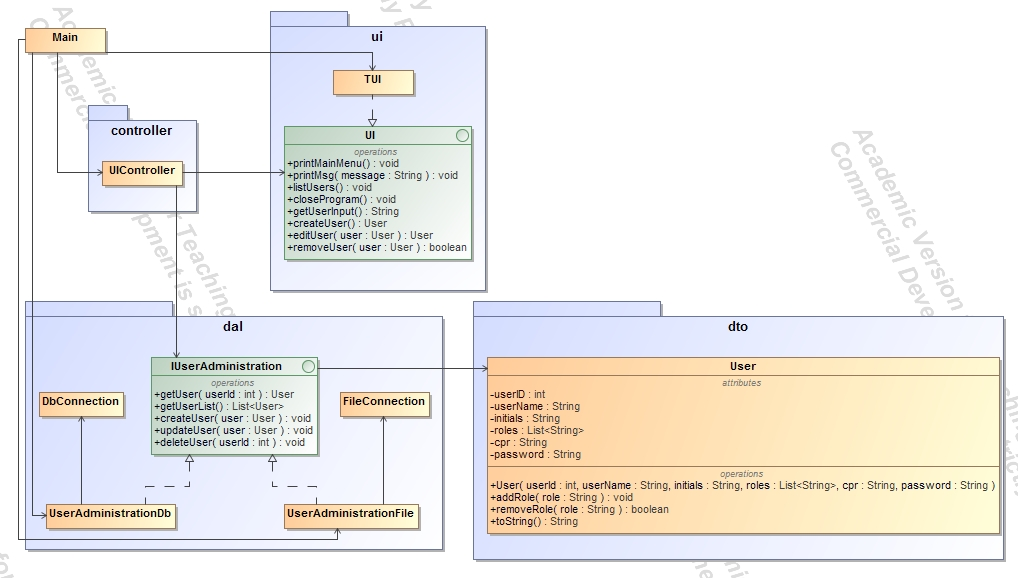
\includegraphics[width=1.4\paperwidth,angle=90]{diagrams/KlasseDiagram.jpg}
\end{figure}
\restoregeometry